\section{Proposed Method}
\label{sec:method}
\begin{figure*}[th]
	\centering
	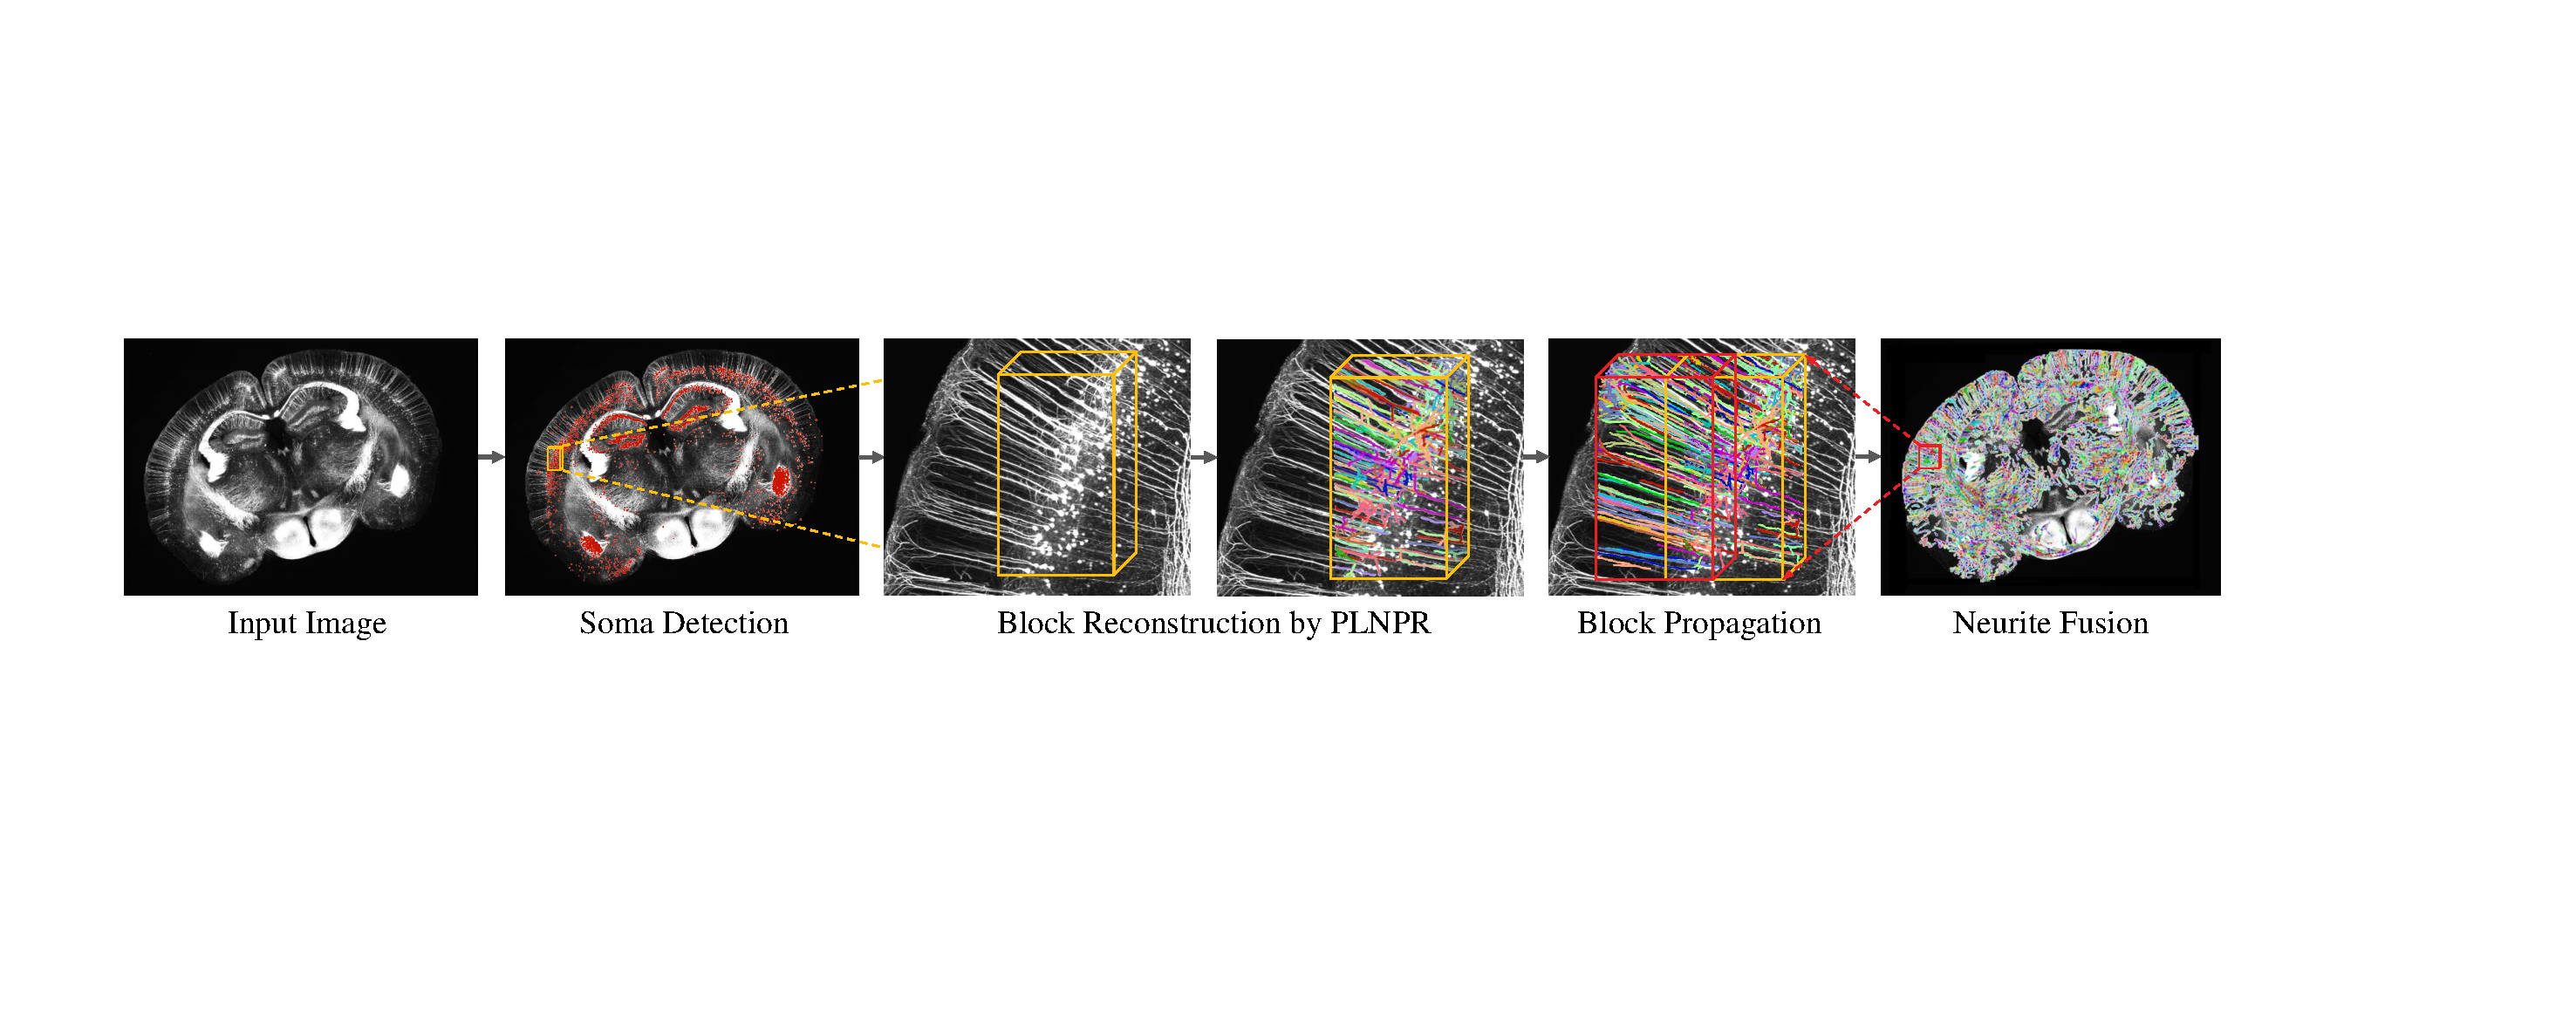
\includegraphics[width=1\textwidth]{./Illustrations/framework_ultranpr.PNG}
	\caption{Diagram of our UltraNPR algorithm for neuronal population reconstruction in a large-scale brain slice.}
	\label{fig:ultra_framework}
\end{figure*}
\md{
Given a  large-scale noisy OM image, we follow a block-by-block reconstruction scheme, as Fig.~\ref{fig:ultra_framework} shows. 
%
The ultra-scale input image may contain billions or even trillions of voxels.
Therefore, we first divide the input image into blocks that are averagely in size of $0.5mm\times0.5mm\times 0.5mm$ with some overlap. 
%
For each block, we first enhance noisy image signals by deep neural network, which is trained by progressive learning from reconstructed neurons using traditional tracing algorithms. Then we reconstruct neuron in each block using the enhanced image. 
%
Since it is more reliably to reconstruct dense neuronal populations starting from somas rather than subtle neurites, our UltraNPR employs an effective block search strategy to trace dense neuronal populations in an adaptive order. 
Finally, we fuse overlapped neurites in adjacent blocks to reconstruct complete neuronal populations for the whole large-scale image.}

\subsection{PLNPR for Robust Neuron Reconstruction}
%\subsection{Unsupervised Progressive Learning for Neuronal Population Reconstruction}
\label{sec:PLNPR}



To reconstruct neurons in a noisy OM image block, our PLNPR algorithm consists of three key components: a segmentation network, an image enhancement module and a neuron tracing module, as shown in Fig.~\ref{fig:framework}. 
%
The segmentation network is designed to extract neuron voxels from noisy and complex backgrounds.
Compared with existing segmentation networks are trained with dense voxel-wise annotations for strong supervision, we use pseudo labels that are generated using traditional neuron tracing methods.
%
In each iteration of segmentation and reconstruction, we apply the NGPST~\cite{Quan2015} as the neuron tracing module to reconstruct neurons from image blocks. 
The tracing module can be replaced by any other tracing method that does not require manual annotations for training.
%
It takes an image block $\mathbf{B}$ as input and reconstructs a neuronal population with separated neurons.
%The intensity $\mathbf{I}(x)$ of a voxel $x$ belongs to $[0,1]$.
From the reconstruction results, we produce a binary mask $\mathbf{M}$ indicating foreground by $\mathbf{M}(x)=1$ and background by $\mathbf{M}(x)=0$ for a voxel $x$.


Given $N$ unlabeled image blocks, we train our segmentation network using the neuron masks $\{\mathbf{M}_i, i=1,\cdots,N\}$ generated from the neuron tracing module.
%
The output of the neuron segmentation network is a 3D probability map $\mathbf{P}$, which is computed by a voxel-wise softmax activation function. $\mathbf{P}(x)\in [0,1]$ indicating the probability of a voxel $x$ to be a neuron part.


Then, by fusing the predicted probability map with the raw signals, the image block is further enhanced in order to preserve both local signals and global structures simultaneously.
When the enhanced block is fed into the neuron tracing module, more complete neuronal populations can be reconstructed and provide better pseudo labels for the next iteration of network training. 
%
Based on the iterative learning process, the powerful DNNs and tracing methods mutually complement and promote each other to gradually improve the neuron reconstruction performance.

\delete{

Then, instead of using a binary mask of the segmented voxels, we employ a probability map predicted by the network and integrate it with the raw image intensities in order to simultaneously preserve the global neuron structure and local neurite details.
After that, a neuron tracing module is applied to reconstruct neurons from the enhanced image block.
Instead of acquiring annotations with huge human efforts, 
we progressively train the segmentation network with the reconstructed neurons inferred from conventional tracing methods as labels, and improve the reconstruction results from better neuron segmentation. 
%Based on the iterative learning process, the powerful DNNs and tracing methods mutually complement and promote each other to gradually improve the neuron reconstruction performance.
}


\begin{figure*}[th]
	\centering
	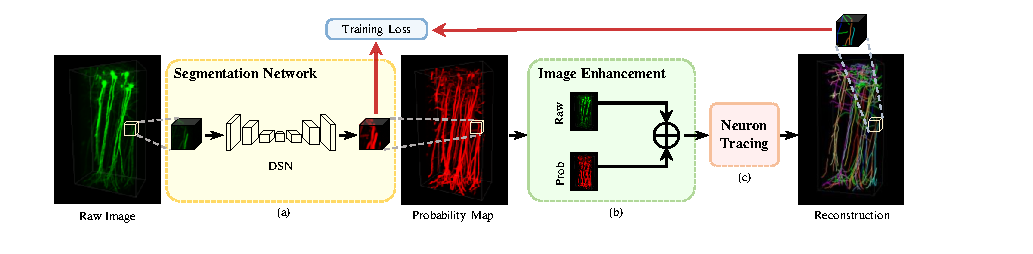
\includegraphics[width=1\textwidth]{./Illustrations/framework2.pdf}
	\caption{Diagram of our progressive learning algorithm for neuron reconstruction in an image block. (a) The segmentation network extracts neuron signals from the raw image. (b) The output probability map is employed to enhance the raw image in order to preserve both global structures and local signal details, which facilitates the neuron tracing module (c) for more complete neuronal population reconstruction. To train the segmentation network, we use the reconstructed neurons as pseudo labels (red arrows), and iteratively refine the network learning and neuron reconstruction with a set of images. The black arrows show the reconstruction pass from an image during testing.}
	\label{fig:framework}
\end{figure*}



%\subsubsection{Progressive Learning without Annotations}
%\label{sec:PL}


\subsubsection{DNN for 3D Neuron Segmentation}
\label{sec:network}
 
Extracting neuron voxels from image blocks is not a trivial problem since the size, morphology and intensity of neurons vary significantly.
In recent years, many 3D DNNs, such as 3D U-Net~\cite{Cicek2016}, 3D DSN~\cite{Dou2017} and DenseVoxNet~\cite{Yu2017} have demonstrated an outstanding capability in various biological and biomedical image segmentation tasks.
Therefore, we take advantage of 3D segmentation networks to extract more representative features to meet the challenges of neuron segmentation.
In this work, we extend the 3D DSN~\cite{Dou2017} as our neuron segmentation network to balance the performance and computation burden.

\delete{
3D DSN consists of convolutional layers, pooling layers and deconvolutional layers, all in 3D fashion. The convolutional layers and pooling layers act as feature extractor, while the deconvolutional layers followed by softmax layer aim to up-sample the feature maps to the same size as the input. To further boost the information flow within the network, two more branches are employed to connect the shallower layers to the output layer. These connections strengthen the gradient propagation, stabilize the learning process, and further taps the potential of the limited training data to learn more discriminative features. %Please refer to~\cite{Dou2017} for more details.
}

Although the original 3D DSN has achieved excellent performance for 3D organ segmentation~\cite{Dou2017}, it is still prone to overfitting in our case due to the limited training data. 
We employ the Dropout~\cite{Srivastava2014} technique during training to learn more robust features that better generalize to new data.
In each convolutional layer, the dropout with a rate of $0.5$ is applied in our network. 



Another challenge of training 3D DNN is the memory limitation because the 3D feature images are huge with respect to the input size. Therefore, for each input image block, we crop a group of small cubes in size of $160\times 160\times 160$ with $30\%$ overlaps, and set batch size to 1 during training. 
%
To have the same physical resolution with the lateral dimension in OM image blocks, voxels in the axial dimension are interpolated after the imaging process. However, this interpolation makes the image quality along different dimensions inhomogeneous. 
Therefore, a random transposition process is employed for each cube as data augmentation for network training.

%Correspondingly, at the test time, we stitch these overlapped probability cubes together using average blending to get a probability map in the same size with the input block.

In addition, the volume of neuron (foreground) voxels is usually much smaller than that of background in an OM image.
To cope with this imbalance problem, a data balancing technique is introduced for network training.
Specifically, when computing the training loss, we only consider the neuron voxels and a certain portion of background voxels, which is randomly selected as non-neuron samples.
The number of non-neuron voxels used for training is set as $10$ times that of neuron voxels.

 

\subsubsection{Image Enhancement}
\label{sec:enhancement}

After training the segmentation network using pseudo labels, we use the trained model to predict a probability map each image cube. 
By averaging the probabilities of the overlapped voxels between adjacent cubes, we can obtain the probability map $\mathbf{P}$ for the entire block $\mathbf{B}$.
Each element in $\mathbf{P}$ indicates the probability that the corresponding voxel in $ \mathbf{B} $ belongs to the neuron.
To utilize the probability map, one natural way is to reconstruct neurons directly from it.
However, since the pseudo labels are not as accurate as manual annotations, 
especially at the early iterations, some local details might lose in the probability map. Therefore, we employ an enhanced representation by fusing the probability map and the raw image block, in order to keep detailed structures and suppress noise signals effectively.
Specifically, a new probability map $\widetilde{\mathbf{P}} $ is first constructed by linearly mapping the value range of $ \mathbf{P}\in [0,1] $ to the value range $[{b}_{min}, {b}_{max}]$ of $\mathbf{B}$.
\begin{equation}
\widetilde{\mathbf{P}}(x) = ({b}_{max}-{b}_{min})\mathbf{P}(x).
\end{equation}


Then, based on the raw signals in block $\mathbf{B}$ and the probability map $\widetilde{\mathbf{P}}$, an enhanced block $\mathbf{E}$ is computed as
\begin{equation}
\mathbf{E}(x) = \alpha\widetilde{\mathbf{P}}(x) + (1-\alpha)\mathbf{B}(x),
\label{equ: enhance}
\end{equation}
where $\alpha\in [0,1]$ is a weight to control the contributions of voxel $ x $ in the original intensity and the probability map. By feeding the enhanced blocks to the neuron tracing module, neuronal populations can be reconstructed more completely.


With more reliable reconstruction results for supervision, the segmentation network could be further trained to learn more discriminative and representative features for producing probability maps, which in turn benefits the tracing module to reconstruct neurons in the next iteration.
%Our system progressively improves the neuron reconstruction performance by combining conventional tracing methods and DNNs without any manual annotations.

As shown in Fig.~\ref{fig:ngps}(a), due to the noises and low contrast in the raw image block, the intensity of neuron voxels is inhomogeneous, which makes some neurons subtle.
At first, by feeding the raw image to the conventional method~\cite{Quan2015}, a neuronal population can be reconstructed. However, compared to the ground truth (GT) shown in Fig.~\ref{fig:ngps}(k), the reconstructed neuronal population is incomplete and many neurites are missing, as Fig.~\ref{fig:ngps}(g) shows.
Then, by utilizing the pseudo labels derived from imperfect reconstruction, the segmentation network can be trained to learn features for global trajectories. Fig.~\ref{fig:ngps}(b) shows the predicted probability map, which demonstrates the enhanced trajectories.
With more iterations of neuron reconstruction and network training, more distinctive and long-range trajectory features can be progressively captured by the network, as shown in Fig.~\ref{fig:ngps}(c)(d)(e).
By combining the original image intensities with the predicted probability map, both local signal details and global trajectories are well preserved in the enhanced block, as Fig.~\ref{fig:ngps}(f) shows.
Iteration by iteration, the completeness and accuracy of neuron reconstruction are progressively improved, as shown in Fig.~\ref{fig:ngps}(h)(i)(j).


\begin{figure}[t]
	\centering
	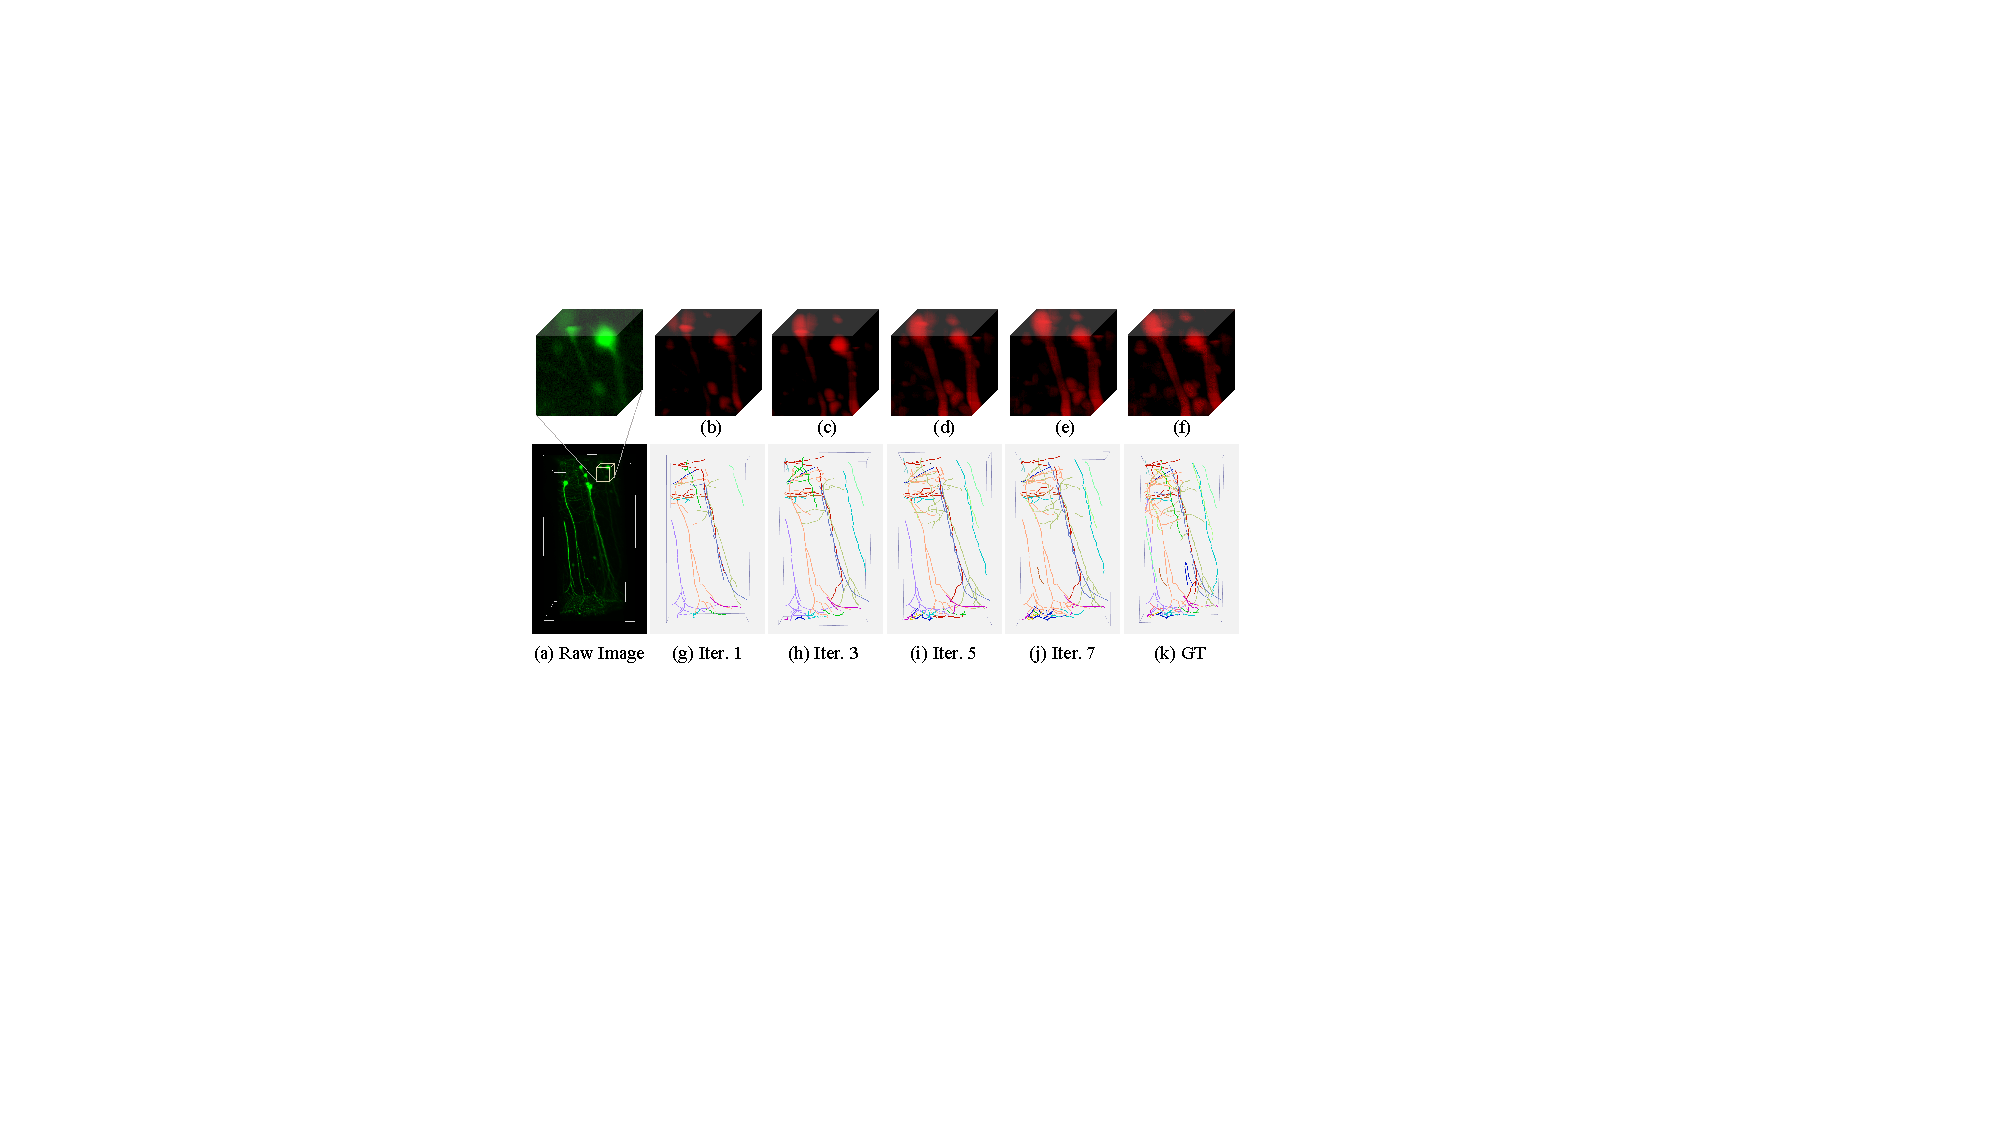
\includegraphics[width=1\columnwidth]{./Illustrations/ngps.pdf}
	\caption{
		Our progressive learning technique gradually improves the segmentation network to extract neuron signals from (a) raw image which has noises and low contrast. (b)(c)(d)(e) The probability maps generated by the segmentation network at different iterations. (f) Combing the probability map and the raw intensity, the enhanced block preserves both global trajectory and local details. (g)(h)(i)(j) More and more complete and accurate reconstruction of the neuronal populations can be obtained with more iterations. (k) The manually labeled neurons are shown for comparison. Separated neurons are shown in different colors.}
	\label{fig:ngps}
\end{figure}
%

\subsection{Large-scale Neuronal Population Reconstruction}
\label{sec:UltraNPR}



Our PLNPR enhances the image signal and traces neurons for each image block.
However, for a ultra-scale OM images consisting of a large number of blocks, neurons usually exist across multiple blocks. 
Therefore, \md{an effective stitching process} is needed to reconstruct complete neuronal populations. 
%
As somas are where signals from the dendrites are joined and pass on, the blocks that contains somas are the most probable locations to start the tracing.
We start from reconstructing neurons in the blocks where somas can be detected and then trace the neurons in neighboring blocks.  
%
Our UltraNPR consists of four key components: a soma detection module, a local reconstruction module, a block search module, and a neurites fusion module, as shown is~\ref{fig:ultra_framework}.
\xj{TODO: ORDER}
\delete{
%At first, the large-scale image is divided into overlapped 3D blocks of the same size. 
%The overlap between adjacent blocks is introduced to avoid false continuation and increase the robustness of the reconstruction.
The soma detection module is used to detect somas from each block.
The local reconstruction module is based on our PLNPR algorithm to reconstruct neurons from low-quality image blocks.
To reconstruct a large-scale image block by block,  we repeatedly apply the block search module to determine what the next block needs to be reconstructed. 
Finally, the neurites fusion module is applied to obtain a complete and continuous reconstruction from adjacent blocks.
}


\subsubsection{Initial Soma Detection}
\label{sec:soma}

In order to detect somas in a ultra-scale image efficiently, we apply the soma detection algorithm~\cite{Quan2013} on each block separately. 
%
For each block $B_{i}$, we get a set of somas $\hat{S}_i = s_{ik}, k=1,\ldots,M_{i} $. 
%Each soma $ s_{ik} $ is represented by its center $ (x,y,z) $ and radius $ r $.
Due to the overlap between blocks, somas in the overlapped area would be detected repeatedly.
We merge the overlapped somas in adjacent blocks by averaging their position and radius to deal with this over-detection problem.
After that, we get a set of somas $ \mathbf{S} $ in the large-scale image, \md{as shown in Fig.~{4} of the supplementary file.}
%The soma detection results from the large-scale image are visualized in Fig.~{4} of the supplementary file.
%These somas are also used to define the initial blocks for neuron reconstruction in the next step.


\subsubsection{Block Search and Local Reconstruction}
\label{sec:trace}

%Since the raw image is too large to directly load it into computer memory before reconstruction, we reconstruct the neuronal population block by block.
%
At the beginning, each block $B_{i}$ is initialized with a flag $ f_i = 0$ to indicate that it has not been reconstructed.
%
After soma detection, if a block $ B_{i}$ contains somas, we apply our PLNPR to reconctruct neurites $ N_{i} $ from it, and set $flag(B_{i})= 1 $ to indicate that it has been reconstructed.
%
For the remaining unreconstructed blocks, we compute the number of its neighboring blocks that have been reconstructed. 
The unreconstructed block $B^*$ with the largest number of neighboring reconstructed blocks is selected for reconstruction next.
%
Though NGPST can perform neuron tracing without any somas, it typically fails to separate neurons with dense neurites, as shown in Fig.~\ref{fig:ngpst_pseudosoma}(a).
%
We follow the structure of the reconstructed neurons in the blocks that have been traced by set the neurite tips as pseudo somas for NGPST in the unreconstructed block.
%
More specifically, for each neighboring reconstructed block of $ B^* $, we collect the neuronal compartments that are close to the boundary of $ B^* $, and use them as the pseudo-somas for growing the neuronal structure in $B^*$.
%Since these compartments typically indicate the continuity of the structure of neurons,  we call them as terminal tips and use them as the pseudo-somas for growing the neuronal structure in $ B^* $.
After that, we get its neurites set $ N^* $, and set $ flag(B^*) = 1 $.
%
This block search and reconstruction process continues iteratively until all blocks have been reconstructed.


\md{Fig.~\ref{fig:blocksearch} shows the procedure of our iterative local reconstruction. the order of propagation, comparison between NGPST with/without neurite tips as pseudo somas. }

\begin{figure*}[t]
	\centering
	%\vspace{1cm}
	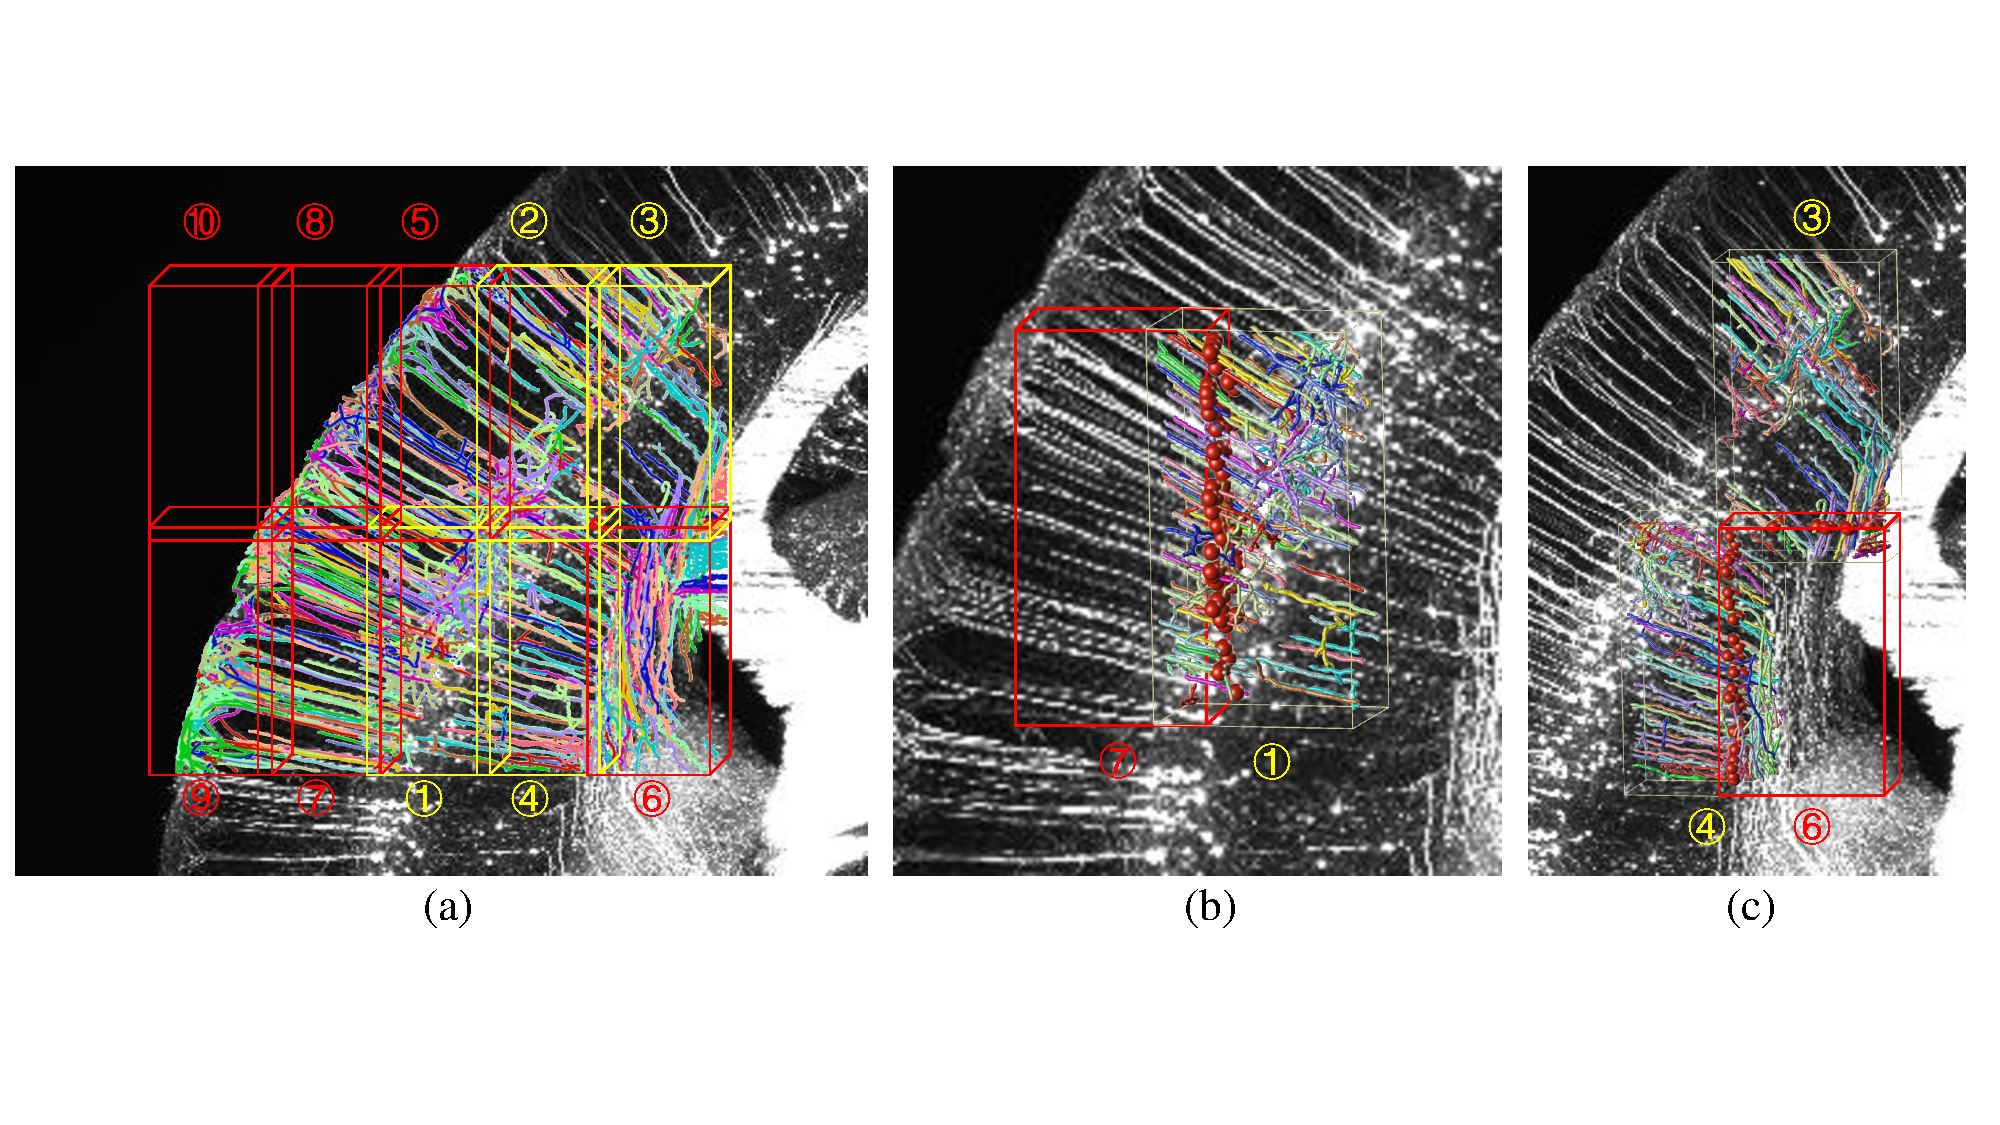
\includegraphics[width=1\textwidth]{./Illustrations/ultranpr_block_search2.pdf}
	\caption{An example of the iterative block reconstruction.  (a) }
	\label{fig:blocksearch}
\end{figure*}

\begin{figure}[t]
	\centering
	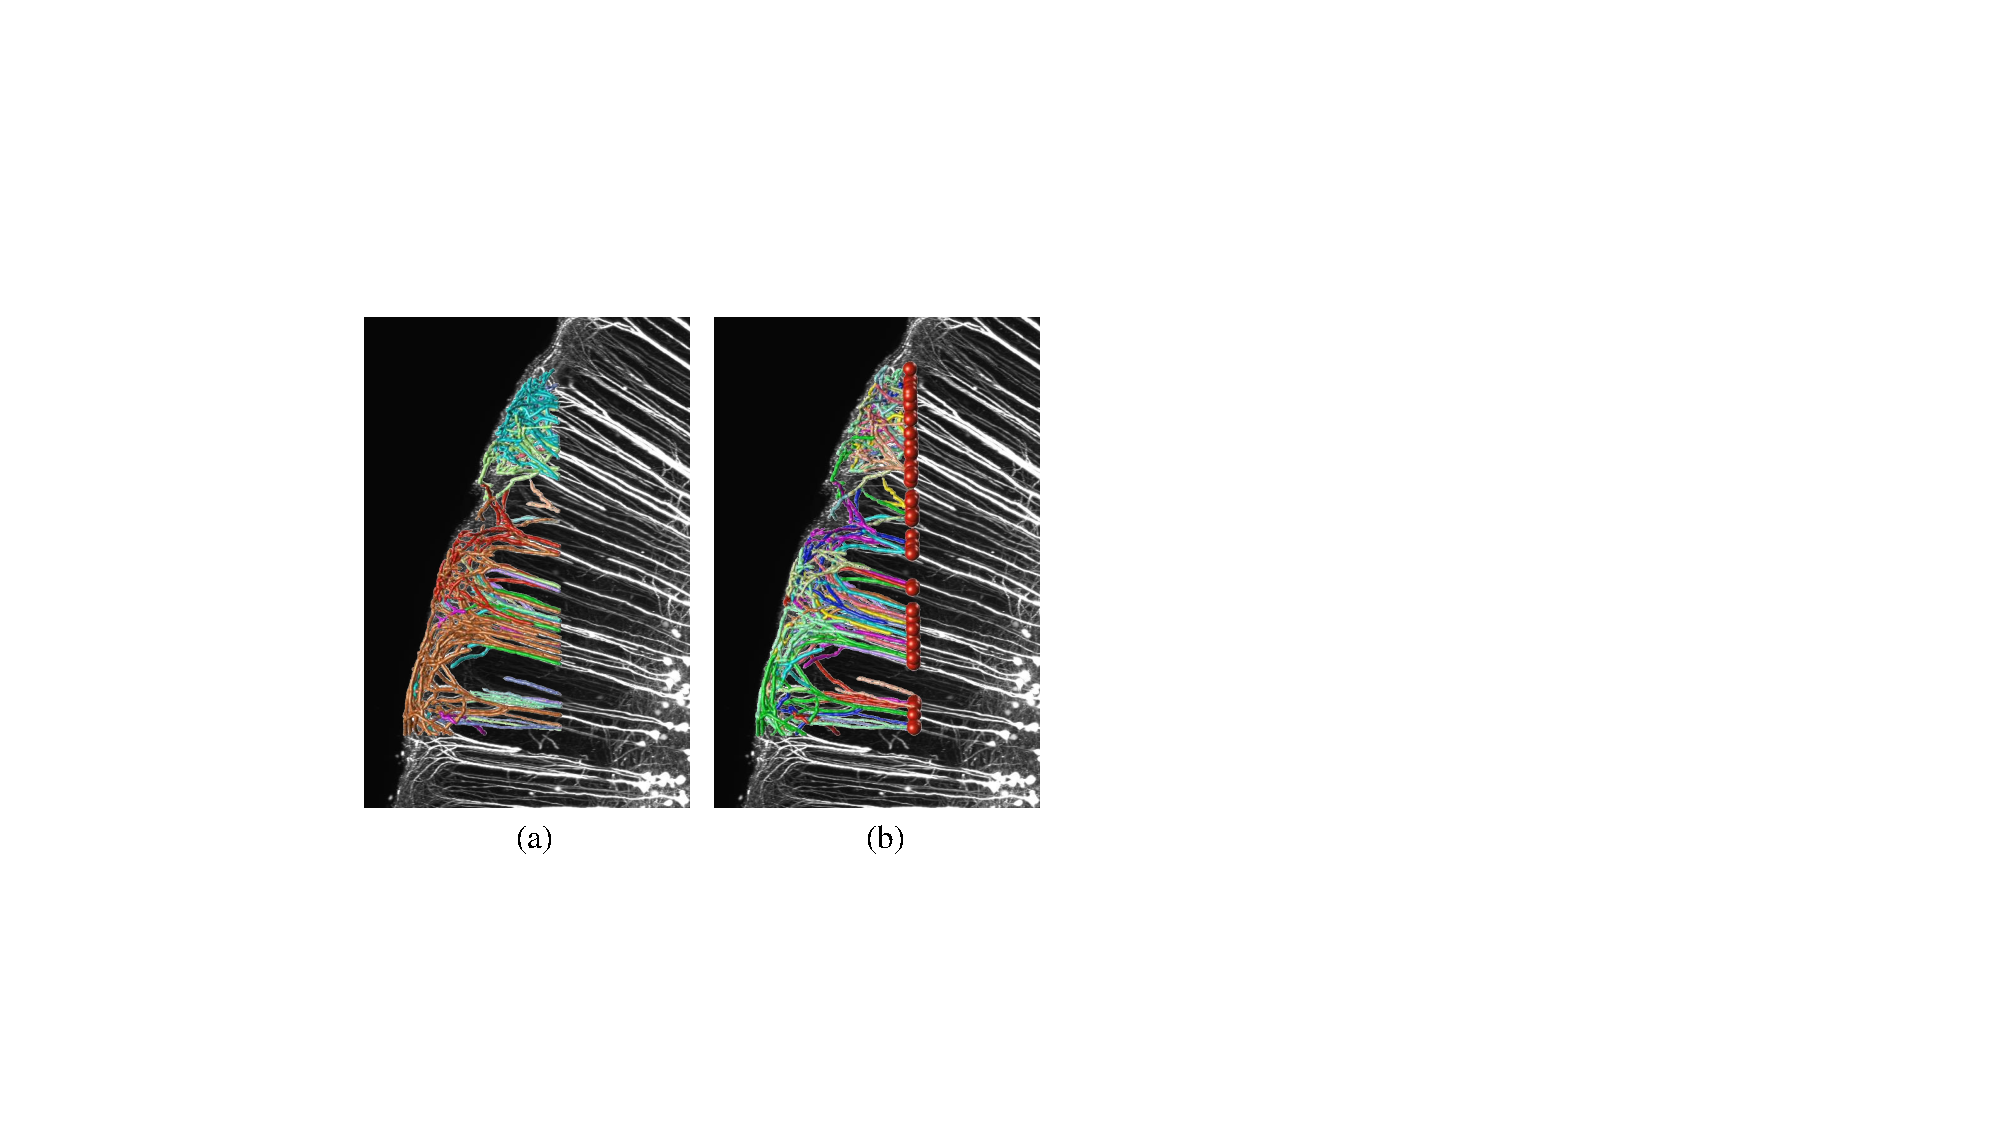
\includegraphics[width=1\columnwidth]{./Illustrations/ngpst_pseudosoma.pdf}
	\caption{Comparison of neuronal population reconstruction on an enhanced image block. (a) Using NGPST without using neurite tips as pseudo somas. 	(b) Using NGPST with neurite tips as pseudo somas. Separated neurons are shown in different colors. }
	\label{fig:ngpst_pseudosoma}
\end{figure}

\subsubsection{Neurites Fusion from Adjacent Blocks}
\label{sec:fusion}

Since neurons would be split into fragmented neurites when dividing the raw image into blocks, neurites from adjacent blocks need to be correctly connected, and the connection should be as continuous and smooth as possible.
\md{Given two overlapped blocks $\mathbf{B}_a$ and $\mathbf{B}_b$, and their reconstructed neurite sets $\mathcal{N}_a$ and $\mathcal{N}_b$, for each neurite ${N}_{ai}$, we look for the neurite ${N}_{bj}$ which has the largest overlapping volume with ${N}_{ai}$. If the overlapped volume between them is larger than a threshold $\delta_{ovlp}$, we fuse these two neurites together to get a smooth and complete reconstruction.} 
\xj{So you fuse the whole neurites together?}
\delete{
As fragmented neurites in the overlapping area may belong to different neurons, we first match them \xj{whom?} by comparing the overlapping region between every two neurites from adjacent blocks.Then, the matched neurites are fused to get a continuous and smooth reconstruction. \xj{This matching process does not matter with different neurons..}
}

However, directly assembling matched neurites would cause over-tracing and topological discrepancy, as shown in Fig.~\ref{fig:overlap_discrepancy}.
The over-tracing problem \xj{highlight the problem in the figure} is caused by the overlap between blocks when the respective neurites from these blocks are assembled.
The topological discrepancy \xj{highlight the problem in the figure} is mainly caused by the lack of context information for tracing methods, which makes the reconstruction near the block boundary often inaccurate and unreliable.
But this region is inside the adjacent block due to the overlap between them, which means substantial context information of this region can be provided to the tracing methods and leads to a better reconstruction.
Therefore, when assembling two matched neurites from adjacent blocks, we only consider neuronal compartments which are not near the boundary of the corresponding block. 
\xj{highlight the boundary area to distinguish with the block. }

\begin{figure}[th]
	\centering
	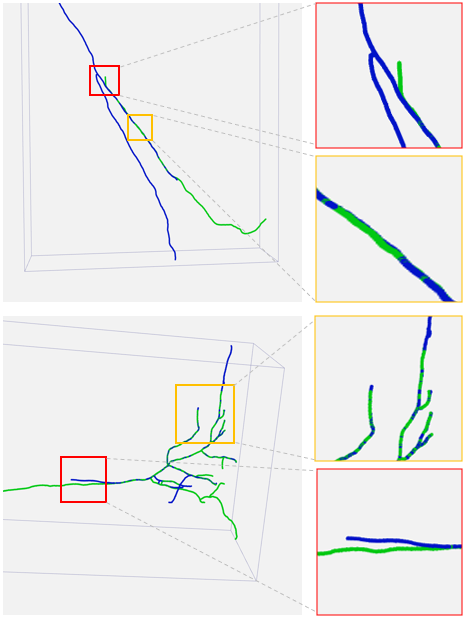
\includegraphics[width=1\columnwidth]{./Illustrations/neuorns_fusion5.png}
	\caption{
		Two examples of over-tracing (yellow) and topological discrepancy (red) errors when assembling two overlapped neurites. These reconstructions are shown in skeleton mode for better visualization. \xj{Show all neurites in two blocks.}}
	\label{fig:overlap_discrepancy}
\end{figure}

\begin{figure}[t]
	\centering
	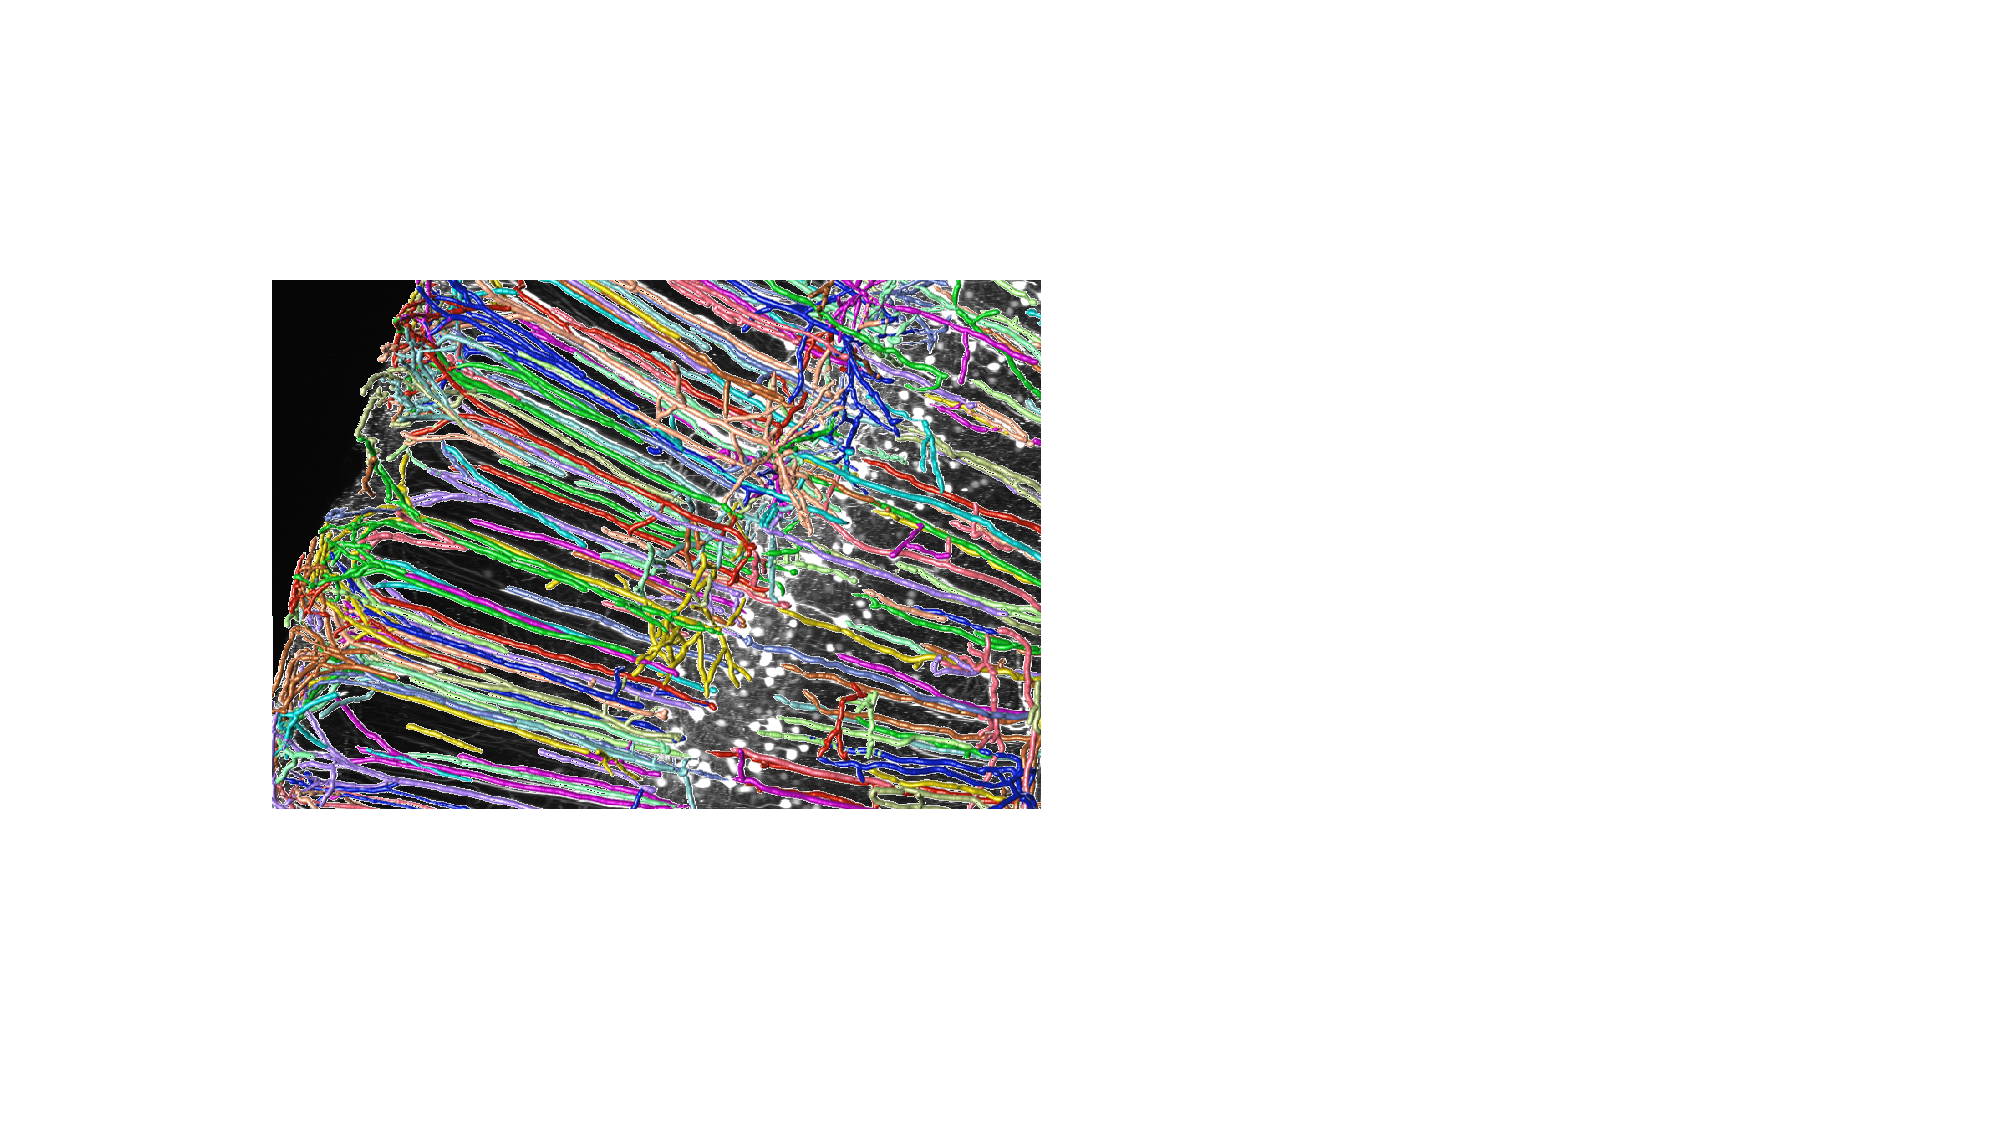
\includegraphics[width=1\columnwidth]{./Illustrations/trace_four_blocks2.pdf}
	\caption{One example of reconstructing neuronal populations from four adjacent blocks using our method. We can observe that, the fragmented neurites from adjacent blocks are assembled continuously and smoothly.}
	\label{fig:reconstruct_blocks}
\end{figure}

\xj{What is the key insight of our fusion algorithm? Fusion order or blending weight or anything? }
Based on the above observations, a fusion algorithm is designed to assemble the matched neurites.
For two matched neurites, we select the longer one as the reference neurite $\mathcal{N}_A$, and merge the other neurite $\mathcal{N}_B$ to the reference neurite.
%
For each branch $\mathcal{H_B}$ in neurite $\mathcal{N_B}$, we search in neurite $\mathcal{N_A}$ to see if there is a branch $\mathcal{H_A}$ that overlaps with it.
\xj{Do you have order for the branches? for root to leaf or leaf to root? say, if you merge a branch in the middle, what happens for all its children or parent branch?  }
%

Firstly, we remove the neuronal compartments in branch $\mathcal{H_A}$ and branch $\mathcal{H_B}$ that near the boundary of the corresponding block, and all branches that are connected to the removed compartments will also be removed. Here, this distance is set to be $70$ voxels.
\xj{What distance? distance between what? how do you compute the distance?}

Secondly, for each neuronal compartment in branch $\mathcal{H_B}$, if there are compartments of branch $\mathcal{H_A}$ around it, it will be removed; otherwise, it is considered to be valid. The searching radius is empirically set to be $10$ voxels.
\xj{what is a compartment in a branch? it is necessary to show a figure to visualize a neurite, a branch, a compartment.   }
\xj{Where is the searching radius used? Using a radius, what is the center? }


 
Thirdly, the first compartment \xj{what do you mean by "first"?} in the modified branch $\mathcal{H_B}$ is connected to $\mathcal{H_A}$ by searching the nearest compartment in branch $\mathcal{H_A}$. 
 
When all branches $\mathcal{H_B}$ overlapping with the neurite $\mathcal{N_A}$ are processed, we can obtain the assembled neurite $\mathcal{N_{AB}}$.
If there are remaining branches $\mathcal{H_B}$ which are not overlapped with neurite $\mathcal{N_A}$, the $\mathcal{N_{AB}}$ will be updated by assembling the remaining branches $\mathcal{H_B}$.

\xj{show the steps of fusion algorithm and then the fusion results. }


Fig.~\ref{fig:overlap_discrepancy} shows two examples of correcting the over-tracing and topological discrepancy errors by our algorithm.
As shown in Fig.~\ref{fig:reconstruct_blocks}, the neuronal population from four adjacent blocks are successfully reconstructed from the noisy images by our UltraNPR method and the fragment neurites in adjacent blocks are assembled continuously and smoothly.
%It can be seen that the neuronal population is successfully reconstructed from the noisy images and the fragment neurites in adjacent blocks are assembled continuously and smoothly.
%The overall ``UltraNPR"" algorithm can be found in Algorithm~\ref{alg:reconstruction}.


